% Provenance (never printed): see sources/outline_sources.md (Year 1: morphology,
% gravity, heat flow and seismicity of a subduction zone; accretionary and erosive
% margins; slab geometry; volcanic arcs). Kuril map, section and numbers from
% figdata/bachelor-1/slab_seismicity.py; exercise and problem values in the Book 3
% scratch calculator calc/ch14.py.
\chapter{Les marges actives}\label{ch:b1:active-margins}

Le 11 mars 2011, à 14 h 46 heure locale, la limite de plaques au large du nord-est du Japon
s'est rompue sur quelque \qty{400}{km} le long de la fosse et sur \qty{150}{km} vers le bas de son \omterm{def:b1:geological-maps:attitude}{pendage}.
La faille a glissé de jusqu'à 50 à \qty{60}{m}, surtout en amont du \omterm{def:b1:geological-maps:attitude}{pendage} par rapport à
l'hypocentre, vers la fosse du Japon~; à terre, la côte s'est déplacée horizontalement et
s'est affaissée. La plaque qui plonge là, la plaque pacifique, descend sous
le Japon le long d'un plan que les séismes dessinent jusqu'à des centaines de kilomètres~;
et là où ce plan se trouve à une centaine de kilomètres de profondeur, une ligne de volcans
court parallèlement à la côte. Ce chapitre lit une telle marge à partir de sa forme,
de sa pesanteur, de son flux de chaleur et, surtout, de ses séismes.
% ledger: usgs:tohoku, wada:decoupling

\begin{recall}
La \omterm{def:b1:layered-earth:lithosphere}{lithosphère} océanique replonge dans le \omterm{def:b1:layered-earth:layers}{manteau} aux zones de subduction, marquées par
des fosses et par des zones inclinées de séismes, et la vieille \omterm{def:b1:layered-earth:lithosphere}{lithosphère} coule sous
son propre poids (livre~2, année~11)~; l'eau de la plaque qui plonge abaisse la
température de fusion du \omterm{def:b1:layered-earth:layers}{manteau} au-dessus d'elle (livre~2, année~12). La chaleur diffuse
sur une distance $L$ en un temps de l'ordre de $L^2/\kappa$ (\cref{ch:b1:heat-budget})~;
une plaque infinie de masse volumique $\rho$ et d'épaisseur $h$ attire avec $2\pi G\rho h$
(\cref{ch:b1:isostasy-gravity})~; les plaques se déplacent autour de \omterm{def:b1:plate-kinematics:euler-pole}{pôles d'Euler}
(\cref{ch:b1:plate-kinematics})~; le flux de chaleur du plancher océanique décroît comme
l'inverse de la racine carrée de son âge (\cref{ch:b1:rifts-ridges-margins}).
\end{recall}

\section{L'anatomie d'une marge active}\label{sec:b1:active-margins:anatomy}

\begin{definition}[Marge active, fosse océanique, avant-arc, bassin d'arrière-arc]\label{def:b1:active-margins:active-margin}
Une \emph{marge active}\index{marge active} est une limite de plaques convergente où
la \omterm{def:b1:layered-earth:lithosphere}{lithosphère} océanique plonge sous une autre plaque, soit sous un
continent, soit sous une autre plaque océanique. Une \emph{fosse
océanique}\index{fosse oceanique@fosse océanique} est la dépression longue, étroite et en V du
fond marin le long de laquelle la plaque qui plonge fléchit vers le bas sous l'autre.
L'\emph{avant-arc}\index{avant-arc} est la partie de la plaque chevauchante comprise entre la
fosse et la ligne de volcans. Un \emph{bassin d'arrière-arc}\index{bassin d'arriere-arc@bassin d'arrière-arc}
est un bassin derrière les volcans, du côté opposé à la fosse, où la
plaque chevauchante est étirée et où de la nouvelle \omterm{def:b1:rifts-ridges-margins:oceanic-crust}{croûte océanique} peut se former.
\end{definition}

Les fosses sont les endroits les plus profonds des océans, et le plus profond de tous est
l'abysse du Challenger, dans la fosse des Mariannes. À travers la fosse des Kouriles le fond passe
d'environ \qty{5200}{m} sur la plaine abyssale à \qty{8700}{m} à l'axe,
soit quelque \qty{3.5}{km} plus bas, et la fosse n'est large que de dizaines de kilomètres
(figure de la \cref{sec:b1:active-margins:gravity-heat}). Les marges convergentes
de la Terre mesurent environ \qty{55000}{km} au total~; dans un modèle numérique des
limites de plaques les limites de subduction totalisent environ \qty{51000}{km},
contre environ \qty{67000}{km} de dorsales d'expansion.
% ledger: data:b3-grav-kuril (trench_gravity.py values), stern:subduction, data:pb2002 (ridge_budget.py)

Du côté océan de la fosse la plaque se soulève légèrement avant de plonger, en un large et
bas bombement externe. Là la plaque est fléchie, et sa partie supérieure est étirée~:
des séismes de faille normale frappent les bombements externes. La largeur du bombement externe
correspond à la flexion d'une plaque élastique~; cette flexion de la \omterm{def:b1:layered-earth:lithosphere}{lithosphère}
est étudiée au livre~5. La fosse elle-même est l'endroit où le poids de la
plaque dense qui plonge tire son bord avant vers le bas.

\begin{definition}[Panneau plongeant]\label{def:b1:active-margins:slab}
Le \emph{panneau plongeant}\index{panneau plongeant} est la partie de la plaque
qui plonge qui est déjà descendue dans le \omterm{def:b1:layered-earth:layers}{manteau}~: une feuille de \omterm{def:b1:layered-earth:lithosphere}{lithosphère} océanique,
avec sa \omterm{def:b1:layered-earth:layers}{croûte} au-dessus, inclinée sous la plaque chevauchante de
la fosse jusqu'à des profondeurs de plusieurs centaines de kilomètres.
\end{definition}

La plaque chevauchante est découpée en bandes parallèles à la fosse
(figure ci-dessous)~: l'\omterm{def:b1:active-margins:active-margin}{avant-arc}, souvent avec un tas de
sédiments raclés à son front et un bassin sédimentaire derrière~; l'\omterm{def:b1:active-margins:volcanic-arc}{arc
volcanique}~; et, derrière certains arcs, un \omterm{def:b1:active-margins:active-margin}{bassin d'arrière-arc} et un arc plus ancien, éteint,
au-delà. Entre le panneau et la plaque chevauchante se trouve un coin de
\omterm{def:b1:layered-earth:layers}{manteau}, entraîné vers le bas le long du dessus du panneau.

\begin{omfigure}
\begin{tikzpicture}[x=0.01667cm, y=0.01667cm, font=\scriptsize,
  lbl/.style={fill=white, fill opacity=0.8, text opacity=1, inner sep=1pt}]
\begin{scope}
\clip (-150,-330) rectangle (650,55);
% mantle and sea water
\fill[orange!12] (-150,-330) rectangle (650,15);
\fill[omSea!45] (-150,15) rectangle (650,0);
% incoming plate and slab: top dips 25 deg to 50 km, then 45 deg; 100 km thick
\fill[omLithBasalt!55] (-150,4) -- (-80,4) .. controls (-60,7) and (-40,7) .. (-25,4) -- (0,0)
  -- (107.2,-50) -- (420,-363) -- (349,-434) -- (48.9,-133.1) -- (-22.1,-100) -- (-150,-100) -- cycle;
\draw[omSea!50!black, line width=1.6pt] (-150,4) -- (-80,4) .. controls (-60,7) and (-40,7) .. (-25,4) -- (0,0) -- (107.2,-50) -- (420,-363);
% overriding plate
\fill[brown!28] (0,0) -- (12,3) -- (45,8) -- (60,10) -- (140,10) -- (150,12) -- (184,12) -- (230,9)
  -- (300,7) -- (395,6) -- (410,3) -- (420,2) -- (430,3) -- (445,6) -- (540,7) -- (560,14) -- (590,14)
  -- (610,10) -- (650,10) -- (650,-60) -- (520,-55) -- (445,-25) -- (420,-15) -- (395,-25) -- (320,-55)
  -- (250,-60) -- (117.2,-60) -- (107.2,-50) -- cycle;
% accretionary prism and forearc basin
\fill[yellow!55] (0,0) -- (12,3) -- (45,8) -- (60,10) -- (60,-28) -- cycle;
\draw[black!45, line width=0.3pt] (14,-3) -- (24,5) (28,-7) -- (38,6) (42,-14) -- (52,8);
\fill[yellow!30] (68,10) -- (132,10) -- (122,4) -- (78,4) -- cycle;
% arc volcano
\fill[black!60] (150,12) -- (167,26) -- (184,12) -- cycle;
% an isotherm: a cold tongue down the slab
\draw[omDef, dashed, line width=0.6pt] (-150,-82) -- (-30,-82) -- (40,-118) -- (300,-318)
  -- (232,-200) -- (150,-112) .. controls (130,-80) and (180,-72) .. (260,-72) -- (650,-72);
% mantle wedge flow
\draw[->, black!60, line width=0.5pt] (600,-130) .. controls (450,-135) and (300,-125) .. (215,-150)
  .. controls (205,-160) and (240,-185) .. (300,-235);
% water and melt
\foreach \x/\z in {150/-93, 172/-115, 194/-137}
  \draw[->, blue!70!black, line width=0.5pt] (\x,\z) -- (\x-6,\z+28);
\draw[red!75!black, line width=0.8pt, decorate, decoration={snake, amplitude=1.2, segment length=6}] (167,-100) -- (167,12);
% earthquakes
\foreach \x/\z in {20/-12, 45/-22, 70/-34, 95/-45, 60/-40, 85/-58, 120/-70, 135/-85, 150/-104,
  165/-112, 185/-140, 205/-150, 225/-175, 248/-195, 270/-216, 290/-242, 312/-262, 330/-282, 350/-300, 365/-318}
  \fill[black] (\x,\z) circle[radius=0.9pt];
% the 100-km level beneath the arc
\draw[black!70, densely dotted] (90,-100) -- (260,-100);
\draw[black!70, densely dotted] (167,12) -- (167,-110);
\end{scope}
\draw[black!70] (-150,-330) rectangle (650,55);
\node[lbl, anchor=south, align=center] at (-85,15) {bombement\\externe};
\node[lbl, anchor=south] at (0,15) {fosse};
\node[lbl, anchor=west] (pr) at (75,-28) {prisme d'accrétion};
\draw[black!70] (pr.west) -- (38,-6);
\node[lbl, anchor=south] at (88,15) {avant-arc};
\node[lbl, anchor=south] at (185,27) {arc volcanique};
\node[lbl, anchor=south] at (420,15) {bassin d'arrière-arc};
\node[lbl, anchor=south] at (575,15) {arc résiduel};
\node[lbl, anchor=west] at (-140,-50) {lithosphère océanique};
\node[lbl, anchor=east] (sl) at (120,-262) {panneau plongeant};
\draw[black!70] (sl.east) -- (205,-262);
\node[lbl, anchor=west] (wb) at (420,-265) {zone de Wadati--Benioff};
\draw[black!70] (wb.west) -- (318,-266);
\node[lbl] at (430,-170) {coin de manteau};
\node[lbl] at (575,-30) {plaque chevauchante};
\node[lbl, anchor=west, text=blue!70!black] at (212,-98) {eau};
\node[lbl, anchor=east] at (88,-100) {\qty{100}{km} de profondeur};
\node[lbl, anchor=west, text=omDef] at (450,-95) {une isotherme};
\node[lbl, anchor=west] at (-140,-300) {manteau};
\draw[line width=1pt] (500,-310) -- (600,-310) node[midway, above] {\qty{100}{km}};
\end{tikzpicture}
\par\smallskip{\small Une zone de subduction en coupe (schématique~: \omterm{def:b1:layered-earth:lithosphere}{lithosphère} et
panneau dessinés à l'échelle de la barre, relief au-dessus du fond marin très exagéré).
Le panneau plonge doucement sous l'\omterm{def:b1:active-margins:active-margin}{avant-arc} et plus fort en dessous~; l'\omterm{def:b1:active-margins:volcanic-arc}{arc
volcanique} se dresse au-dessus de l'endroit où le dessus du panneau est à environ \qty{100}{km}
de profondeur. Le panneau froid entraîne ses isothermes vers le bas dans le \omterm{def:b1:layered-earth:layers}{manteau} (en tirets~: une
isotherme), et le \omterm{def:b1:layered-earth:layers}{manteau} du coin est entraîné vers le bas le long de lui. Points~:
séismes, sur la limite de plaques près de la fosse et à l'intérieur du panneau en dessous.
L'eau libérée par le panneau monte dans le coin~; le magma monte vers l'arc.}
\label{fig:b1:active-margins:section}
\end{omfigure}

En sommant sur le même modèle numérique, environ \qty{2.7}{km^2} de plancher océanique
descendent chaque année aux limites de subduction, proche des \qty{3.0}{km^2} faits
aux dorsales (\cref{ch:b1:rifts-ridges-margins})~: dans la précision d'un tel
modèle, qui laisse de côté la lente déformation des larges zones de limites de plaques, le
plancher océanique est détruit aussi vite qu'il est fait, et la surface de la Terre
garde sa taille.
% ledger: data:pb2002 (ridge_budget.py: consumed 2.74, made 3.01 km2/yr)

\section{Pesanteur et flux de chaleur}\label{sec:b1:active-margins:gravity-heat}

Felix Vening Meinesz a trouvé les longues et étroites bandes d'\omterm{def:b1:isostasy-gravity:anomalies}{anomalies de pesanteur} négatives
le long des fosses (\cref{ch:b1:isostasy-gravity}). Les satellites les cartographient maintenant
partout en mer. À travers la fosse des Kouriles (figure ci-dessous) l'\omterm{def:b1:isostasy-gravity:anomalies}{anomalie à l'air libre}
monte à environ \qty{40}{\milli\gal} sur le bombement externe, tombe à
\qty{-260}{\milli\gal} sur la fosse, et est de nouveau fortement positive sur
l'\omterm{def:b1:active-margins:active-margin}{avant-arc} et les îles de l'arc.
% ledger: egs:vening-meinesz, data:b3-grav-kuril (trench_gravity.py values: rise 38 mGal at -155 km, low -260 at 0, high 218 at 160 km)

La taille de l'anomalie de la fosse dit comment la fosse est maintenue. Supposons que la fosse,
plus profonde de \qty{3.5}{km} que le plancher qui l'entoure, ne soit pas compensée du tout~:
là où est la fosse, \qty{3.5}{km} de roche de masse volumique d'environ
\qty{2700}{kg.m^{-3}} sont remplacés par de l'eau de mer. D'après la plaque de Bouguer
(\cref{prop:b1:isostasy-gravity:slab}) la pesanteur y serait plus basse de
\[
  2\pi G\,\Delta\rho\,h = 2\pi \times \num{6.674e-11} \times 1700 \times 3500
  \approx \qty{2.5e-3}{m.s^{-2}} = \qty{250}{\milli\gal} .
\]
C'est la taille du minimum observé. Une fosse n'est donc pas en équilibre isostatique~:
c'est une dépression maintenue vers le bas, par la résistance de la plaque fléchie
et par la traction du panneau, contre la poussée du \omterm{def:b1:layered-earth:layers}{manteau} en dessous. (Une
fosse large de dizaines de kilomètres seulement attire moins qu'une plaque infinie, donc
l'eau qu'elle contient donne à elle seule un peu moins que cela~; le reste du déficit
se trouve plus profond, là où toute la plaque fléchie, sa \omterm{def:b1:layered-earth:layers}{croûte} légère comprise, est enfoncée
dans le \omterm{def:b1:layered-earth:layers}{manteau}~: exercice~\ref{exo:b1:active-margins:1}.)

\begin{omfigure}
\begin{tikzpicture}
\begin{axis}[omrecord, name=grav, width=0.86\linewidth, height=4.6cm, xmin=-250, xmax=450,
  ymin=-300, ymax=260, ylabel={air libre (\unit{\milli\gal})}, ylabel style={at={(-0.075,0.5)}}, xticklabels={},
  ytick={-200,-100,0,100,200}, clip=false]
% computed in figdata/bachelor-1/trench_gravity.py; ledger: data:b3-grav-kuril
\addplot[black!30, forget plot] coordinates {(-250,0) (450,0)};
\addplot[omDef, line width=1pt] table[x=x, y=faa] {figdata/out/bachelor-1-trench_gravity-profile.dat};
\draw[black!50, densely dotted] (axis cs:0,-300) -- (axis cs:0,260) (axis cs:164,-300) -- (axis cs:164,260);
\node[font=\scriptsize, anchor=south west] at (axis cs:-240,45) {bombement externe, $+38$};
\node[font=\scriptsize, anchor=west] at (axis cs:12,-262) {fosse, $-260$};
\node[font=\scriptsize, anchor=south west] at (axis cs:200,140) {avant-arc et arc};
\end{axis}
\begin{axis}[omrecord, at={(grav.south)}, anchor=north, yshift=-0.45cm, width=0.86\linewidth, height=4.6cm,
  xmin=-250, xmax=450, ymin=20, ymax=100, ylabel={flux de chaleur (\unit{mW.m^{-2}})}, ylabel style={at={(-0.075,0.5)}},
  xlabel={distance à la fosse, vers la plaque chevauchante (\unit{km})}, clip=false]
% schematic; levels from the ledger: parsons:plate-model (11.3/sqrt(122) x 41.84 = 42.8 mW/m2 for the
% 122-Myr Kuril plate), hyndman:backarc (70-85); the forearc low is drawn without a value (wada:decoupling)
\addplot[fill=omDef!15, draw=none, forget plot] coordinates {(190,70) (450,70) (450,85) (190,85)} -- cycle;
\addplot[omProp!80!black, line width=1pt, smooth, tension=0.5] coordinates {(-250,43) (-60,43) (-10,41) (30,36) (120,36)
  (150,48) (180,76) (230,78) (450,78)};
\draw[black!50, densely dotted] (axis cs:0,20) -- (axis cs:0,100) (axis cs:164,20) -- (axis cs:164,100);
\node[font=\scriptsize, anchor=south west] at (axis cs:-240,44) {vieux plancher, environ 43};
\node[font=\scriptsize, anchor=north] at (axis cs:75,34) {avant-arc~: plus bas};
\node[font=\scriptsize, anchor=south] at (axis cs:320,85) {arc et arrière-arc, 70 à 85};
\node[font=\scriptsize, anchor=north west] at (axis cs:3,99) {fosse};
\node[font=\scriptsize, anchor=north west] at (axis cs:167,99) {arc};
\end{axis}
\end{tikzpicture}
\par\smallskip{\small Pesanteur et flux de chaleur à travers une zone de subduction. En haut~:
l'\omterm{def:b1:isostasy-gravity:anomalies}{anomalie de pesanteur} à l'air libre mesurée par satellite à travers la fosse des Kouriles, le long
de la coupe de la figure de la \cref{sec:b1:active-margins:seismicity}~:
\qty{38}{\milli\gal} sur le bombement externe, \qty{-260}{\milli\gal} sur la
fosse, fortement positive sur l'\omterm{def:b1:active-margins:active-margin}{avant-arc} et les îles. En bas~: le flux de chaleur,
un profil schématique~: environ \qty{43}{mW.m^{-2}} sur le vieux plancher océanique, plus bas
sur l'\omterm{def:b1:active-margins:active-margin}{avant-arc}, 70 à \qty{85}{mW.m^{-2}} en moyenne sur l'arc et
l'arrière-arc. Pointillés~: la fosse et le front volcanique. Données~: modèle marin de
pesanteur de la Scripps Institution of Oceanography (Sandwell et collab., 2014).}
\label{fig:b1:active-margins:profiles}
\end{omfigure}

Le flux de chaleur raconte la même histoire de l'autre côté. Le vieux plancher océanique
qui arrive à une fosse perd peu de chaleur~: environ \qty{43}{mW.m^{-2}} d'après la loi
du \cref{ch:b1:rifts-ridges-margins} pour la plaque des Kouriles, âgée de \qty{122}{\Ma}.
Sur l'\omterm{def:b1:active-margins:active-margin}{avant-arc} le flux est plus faible encore~: le panneau froid en dessous absorbe de la
chaleur par le haut, et le \omterm{def:b1:layered-earth:layers}{manteau} sous l'\omterm{def:b1:active-margins:active-margin}{avant-arc} est froid et stagnant. Sur l'arc
et l'arrière-arc il est élevé, 70 à \qty{85}{mW.m^{-2}} en moyenne, le double du
flux des vieux intérieurs de continents (environ \qty{40}{mW.m^{-2}}). Un \omterm{def:b1:active-margins:volcanic-arc}{arc
volcanique} actif demande un coin de \omterm{def:b1:layered-earth:layers}{manteau} à environ \qty{1200}{\celsius} à quelque
\qty{100}{km} de profondeur~; derrière lui tout l'arrière-arc est chaud, avec une \omterm{def:b1:layered-earth:lithosphere}{lithosphère}
épaisse de seulement 50 à \qty{60}{km} et son \omterm{def:b1:layered-earth:discontinuity}{Moho} à 800 à \qty{900}{\celsius}.
% ledger: parsons:plate-model (11.3/sqrt(122) x 41.84 = 42.8), wada:decoupling, hyndman:backarc
Pourquoi le panneau reste-t-il froid~? Il plonge plus vite qu'il ne peut se réchauffer. Le panneau
des Kouriles de la \cref{sec:b1:active-margins:seismicity} entre à environ
\qty{82}{mm} par an et plonge à \ang{45}~: il atteint \qty{600}{km} après un trajet
de $600/\sin\ang{45} \approx \qty{850}{km}$, en environ dix millions d'années. D'après
l'échelle de temps conductive (\cref{prop:b1:heat-budget:timescale}), la chaleur du
\omterm{def:b1:layered-earth:layers}{manteau} traverse les \qty{50}{km} jusqu'au milieu d'un panneau épais de \qty{100}{km} en
\[
  \tau = \frac{L^2}{\kappa} = \frac{(\qty{5e4}{m})^2}{\qty{e-6}{m^2.s^{-1}}}
  = \qty{2.5e15}{s} \approx \qty{80}{\Ma},
\]
environ huit fois plus longtemps. Le cœur du panneau arrive à \qty{600}{km} presque aussi
froid qu'il l'était à la fosse, et les isothermes sont entraînées vers le bas avec lui, comme le
montre plus haut la coupe d'une zone de subduction.
% values (slab_seismicity.py): vel_normal 81.66 mm/yr, dip 44.9; calc/ch14.py

\section{Séismes et forme du panneau}\label{sec:b1:active-margins:seismicity}

\begin{definition}[Zone de Wadati--Benioff]\label{def:b1:active-margins:wadati-benioff}
Une \emph{zone de Wadati--Benioff}\index{zone de Wadati--Benioff} est la zone inclinée
de séismes qui commence près d'une fosse et s'approfondit sous la plaque chevauchante,
jusqu'à environ \qty{700}{km}~: elle dessine le \omterm{def:b1:active-margins:slab}{panneau plongeant}.
\end{definition}
% ledger: usgs:deepest

Ses séismes sont de deux sortes. Jusqu'à quelques dizaines de kilomètres ils se produisent sur
la limite de plaques elle-même, la faille faiblement inclinée le long de laquelle les deux plaques
glissent l'une contre l'autre~; les plus grands séismes de la Terre, comme celui de 2011
au large du Japon, rompent cette faille. Plus profond, ils se produisent à l'intérieur du panneau, qui seul est
encore assez froid pour stocker des contraintes. Aux plus grandes profondeurs même le panneau devrait
s'écouler plutôt que se rompre, et la façon dont commencent les séismes profonds est encore débattue. Le
séisme le plus profond du catalogue, de magnitude 4.2, a frappé sous la
région du Vanuatu en 2004 à \qty{735.8}{km}. Dans chaque zone de subduction examinée,
la zone est double aux profondeurs intermédiaires~: deux couches de séismes, plus
écartées dans les plaques plus vieilles.
% ledger: usgs:deepest, brudzinski:double, usgs:tohoku

Les îles Kouriles, entre Hokkaido et le Kamtchatka, se trouvent au-dessus d'un panneau que les
séismes dessinent de la fosse jusqu'à plus de \qty{600}{km}. Là la plaque pacifique, âgée d'environ 120 millions d'années
à la fosse, plonge sous la plaque d'Okhotsk
(carte ci-dessous). Les séismes de magnitude 5 ou plus depuis
1976 dessinent le panneau en plan~: les superficiels le long de la fosse, les intermédiaires
sous les îles, les profonds sous la mer d'Okhotsk. Le 24 mai 2013 un
séisme de magnitude 8.3 a frappé à \qty{598}{km} sous la mer d'Okhotsk,
dans le même panneau plus au nord~; il a été ressenti jusqu'à Moscou, à quelque
\qty{6400}{km}.
% values (slab_seismicity.py): age_in 121.8 Myr (median of the cells 100-400 km seaward)
% ledger: data:b3-usgs-kuril, data:b2-seafloor-age, data:pb2002, usgs:okhotsk-2013

\begin{omfigure}
\begin{tikzpicture}
\begin{axis}[x=0.40cm, y=0.598cm, xmin=138, xmax=165, ymin=40, ymax=56,
  axis background/.style={fill=omSea!35}, axis on top,
  xtick={140,145,...,165}, ytick={40,45,...,55},
  xticklabel={$\pgfmathprintnumber{\tick}^\circ$E}, yticklabel={$\pgfmathprintnumber{\tick}^\circ$N},
  tick label style={font=\scriptsize}, grid=major, grid style={gray!25, line width=0.25pt},
  legend style={font=\scriptsize, at={(0.98,0.02)}, anchor=south east, cells={anchor=west}},
  clip=true]
% computed in figdata/bachelor-1/slab_seismicity.py; ledger: data:b3-usgs-kuril, data:gvp, data:pb2002
\addplot[fill=omLithAlluv, draw=black!45, line width=0.2pt, unbounded coords=jump, forget plot] table {figdata/out/bachelor-1-slab_seismicity-map-land.dat};
\addplot[only marks, mark=*, mark size=0.45pt, black!35] table {figdata/out/bachelor-1-slab_seismicity-map-qshallow.dat};
\addlegendentry{moins profond que \qty{70}{km}}
\addplot[only marks, mark=*, mark size=0.8pt, orange!85!black] table {figdata/out/bachelor-1-slab_seismicity-map-qmid.dat};
\addlegendentry{70 à \qty{300}{km}}
\addplot[only marks, mark=*, mark size=1.0pt, omDef] table {figdata/out/bachelor-1-slab_seismicity-map-qdeep.dat};
\addlegendentry{plus profond que \qty{300}{km}}
\addplot[only marks, mark=triangle*, mark size=1.6pt, black, fill=red!70!black] table {figdata/out/bachelor-1-slab_seismicity-map-volc.dat};
\addlegendentry{volcan holocène}
\addplot[black, line width=0.6pt, unbounded coords=jump, forget plot] table {figdata/out/bachelor-1-slab_seismicity-map-trench.dat};
\addplot[fill=black, draw=none, unbounded coords=jump, forget plot] table {figdata/out/bachelor-1-slab_seismicity-map-teeth.dat};
\addplot[omProp, line width=0.8pt, dashed, forget plot] table {figdata/out/bachelor-1-slab_seismicity-map-strip.dat};
\node[font=\scriptsize, fill=white, fill opacity=0.8, text opacity=1, inner sep=1pt] at (axis cs:147,54.3) {mer d'Okhotsk};
\node[font=\scriptsize, fill=white, fill opacity=0.8, text opacity=1, inner sep=1pt] at (axis cs:158.5,44) {plaque pacifique};
\node[font=\scriptsize, fill=white, fill opacity=0.8, text opacity=1, inner sep=1pt] at (axis cs:157.2,55.2) {Kamtchatka};
\node[font=\scriptsize, fill=white, fill opacity=0.8, text opacity=1, inner sep=1pt] at (axis cs:139.7,44.3) {Hokkaido};
\node[font=\scriptsize, fill=white, fill opacity=0.8, text opacity=1, inner sep=1pt, rotate=40] at (axis cs:155.6,46.4) {fosse des Kouriles};
\node[font=\scriptsize, fill=white, fill opacity=0.8, text opacity=1, inner sep=1pt, text=omProp] at (axis cs:146.3,51.4) {coupe};
\end{axis}
\end{tikzpicture}
\par\smallskip{\small La zone de subduction des Kouriles~: séismes de magnitude 5 ou
plus, 1976--2025, colorés selon la profondeur, et volcans actifs durant les dix derniers
mille ans. La fosse (dents sur la plaque chevauchante) et la bande de la
coupe montrée dans la figure suivante (en tirets, \qty{150}{km} de
chaque côté de la ligne de coupe). Données~: catalogue de séismes de l'USGS~; Smithsonian
Global Volcanism Program~; fosse d'après Bird (2003)~; côtes de Natural Earth.}
\label{fig:b1:active-margins:map}
\end{omfigure}

Pour voir le panneau en coupe, on garde les séismes situés à moins de \qty{150}{km} d'une ligne
qui part de la fosse et court perpendiculairement à elle, vers la plaque
chevauchante, et l'on trace chacun à sa distance $x$ le long de la ligne et à sa profondeur $z$
(figure ci-dessous). Les points forment une bande~; la
droite qui la suit le mieux se trouve par les moindres carrés.

\begin{method}[Ajuster le panneau par les moindres carrés]\label{met:b1:active-margins:lsq}
Soit $n$ séismes en $(x_i, z_i)$ à l'intérieur du panneau~:
\begin{enumerate}
  \item calculer les moyennes $\bar x = \frac1n\sum x_i$ et $\bar z = \frac1n\sum z_i$~;
  \item calculer $S_{xx} = \sum (x_i - \bar x)^2 = \sum x_i^2 - n\bar x^2$ et
        $S_{xz} = \sum (x_i - \bar x)(z_i - \bar z) = \sum x_i z_i - n\bar x\bar z$~;
  \item la droite du panneau est $z = a + s x$ avec $s = S_{xz}/S_{xx}$ et
        $a = \bar z - s\bar x$~; son \omterm{def:b1:geological-maps:attitude}{pendage} est $\delta = \arctan s$.
\end{enumerate}
\end{method}

La droite minimise la somme des carrés des écarts verticaux
$F(a, s) = \sum_i (z_i - a - s x_i)^2$, une fonction quadratique de $a$ et $s$
qui est minimale là où les deux dérivées partielles s'annulent. $\partial F/\partial a =
-2\sum (z_i - a - s x_i) = 0$ donne $\bar z = a + s\bar x$~: la droite passe
par le centre des points. En substituant $a = \bar z - s\bar x$,
$\partial F/\partial s = -2\sum x_i\,[(z_i - \bar z) - s(x_i - \bar x)] = 0$~;
puisque $\sum \bar x\,[(z_i - \bar z) - s(x_i - \bar x)] = 0$, cela s'écrit
$\sum (x_i - \bar x)[(z_i - \bar z) - s(x_i - \bar x)] = 0$, c'est-à-dire
$S_{xz} = s S_{xx}$.

Sous les îles Kouriles centrales la bande contient 599 séismes, dont 121
plus profonds que \qty{70}{km}, à l'intérieur du panneau. Les moins profonds sont peu utiles
pour l'ajustement~: ils mêlent la limite de plaques et la plaque qui fléchit, et 147 des
478 sont listés à la même profondeur ronde de \qty{33}{km}. Les 121 plus profonds donnent
\[
  z = -52.7 + 0.996\,x \quad\text{(kilomètres)},
\]
un \omterm{def:b1:geological-maps:attitude}{pendage} de \ang{44.9}, environ \ang{45}, jusqu'au séisme le plus profond de la bande,
\qty{632}{km}. La droite ne passe pas par la fosse~: elle atteint la
surface à \qty{53}{km} de celle-ci vers l'intérieur des terres. Le panneau n'est pas rectiligne~: il quitte la
fosse avec un \omterm{def:b1:geological-maps:attitude}{pendage} plus doux et se redresse sous l'\omterm{def:b1:active-margins:active-margin}{avant-arc}, comme le montrent les
séismes peu profonds au-dessus de la droite.
% values (slab_seismicity.py): n_section 599, n_fit 121, fit_a -52.721, fit_s 0.996397, dip 44.8966,
% max_depth 631.9; 147 of the 478 events of 70 km or less at 33.0 km (section part)

\begin{omfigure}
\begin{tikzpicture}
\begin{axis}[omrecord, omdepth, scale only axis, width=11.25cm, height=8.75cm,
  xmin=-100, xmax=800, ymin=0, ymax=700,
  xlabel={distance à la fosse, vers la mer d'Okhotsk (\unit{km})},
  ylabel={profondeur (\unit{km})}, clip=false,
  legend style={font=\scriptsize, at={(0.02,0.02)}, anchor=south west, cells={anchor=west}}]
% computed in figdata/bachelor-1/slab_seismicity.py; ledger: data:b3-usgs-kuril, data:gvp, data:pb2002
\addplot[only marks, mark=*, mark size=0.7pt, black!30] table[x=x, y=depth, restrict y to domain=0:70] {figdata/out/bachelor-1-slab_seismicity-section.dat};
\addlegendentry{moins profond que \qty{70}{km}}
\addplot[only marks, mark=*, mark size=1.0pt, black!80] table[x=x, y=depth, restrict y to domain=70.01:800] {figdata/out/bachelor-1-slab_seismicity-section.dat};
\addlegendentry{plus profond (ajusté)}
\addplot[omProp, line width=1pt, domain=60:740, samples=2] {-52.721 + 0.996397*x};
\addlegendentry{droite des moindres carrés, pendage \ang{45}}
\addplot[only marks, mark=triangle*, mark size=3pt, omDef, forget plot] coordinates {(0,0)};
\addplot[only marks, mark=triangle*, mark size=3pt, red!70!black, forget plot] coordinates {(163.9,0)};
\draw[black!70, densely dashed] (axis cs:163.9,0) -- (axis cs:163.9,110.6);
\node[font=\scriptsize, anchor=north, text=omDef] at (axis cs:0,-28) {fosse};
\node[font=\scriptsize, anchor=south, text=red!70!black] at (axis cs:175,-8) {front volcanique};
\draw[black!70] (axis cs:166,110.6) -- (axis cs:290,80);
\node[font=\scriptsize, anchor=west, fill=white, fill opacity=0.8, text opacity=1, inner sep=1pt] at (axis cs:290,80) {panneau à \qty{111}{km} sous le front};
\end{axis}
\end{tikzpicture}
\par\smallskip{\small Le panneau des Kouriles en coupe, sans \omterm{def:b1:cross-sections:section}{exagération verticale}~: les séismes de la bande de la carte ci-dessus
à leur distance à la fosse et à leur profondeur. La droite des moindres carrés
passant par les 121 séismes plus profonds que \qty{70}{km} plonge de \ang{45}. Le premier
volcan de la bande, à \qty{164}{km} de la fosse, se dresse au-dessus de l'endroit
où la droite est à \qty{111}{km} de profondeur. Données~: catalogue de séismes de l'USGS~;
Smithsonian Global Volcanism Program~; fosse d'après Bird (2003).}
\label{fig:b1:active-margins:kuril-section}
\end{omfigure}

Un panneau froid est plus dense que le \omterm{def:b1:layered-earth:layers}{manteau} qui l'entoure, et son poids tire la
plaque derrière lui~: c'est la traction du \omterm{def:b1:active-margins:slab}{panneau plongeant} du livre~2, année~11. Sa taille se déduit
de la profondeur du plancher océanique.

\begin{proposition}[Le poids excédentaire d'un panneau]\label{prop:b1:active-margins:slab-weight}
Sous les hypothèses de la \omterm{thm:b1:rifts-ridges-margins:depth-age}{loi profondeur--âge}
(\cref{thm:b1:rifts-ridges-margins:depth-age}), une plaque d'âge $A$ porte, par
unité d'aire, la masse excédentaire
\[
  m = (\rho_m - \rho_w)\bigl(d(A) - d_r\bigr)
    = \frac{2}{\sqrt\pi}\,\rho_m\,\alpha\,(T_m - T_0)\sqrt{\kappa A}
\]
par rapport au \omterm{def:b1:layered-earth:layers}{manteau} à $T_m$. Un panneau de cette plaque, de longueur $L$ selon son \omterm{def:b1:geological-maps:attitude}{pendage}
$\delta$ et non encore réchauffé, a le poids excédentaire $F = g\,m\,L$ par unité de longueur
de fosse, dont $F\sin\delta$ agit le long du panneau.
\end{proposition}

\begin{proof}
Une couche $\mathrm dz$ de la plaque à la température $T$ a la masse
$\rho_m\bigl(1 + \alpha(T_m - T)\bigr)\mathrm dz$ par unité d'aire, c'est-à-dire
$\rho_m\alpha(T_m - T)\,\mathrm dz$ de plus que le \omterm{def:b1:layered-earth:layers}{manteau} à $T_m$. Sommé sur la
plaque, cet excès est $\rho_m\alpha\int_0^\infty (T_m - T)\,\mathrm dz$, dont la
démonstration de la \omterm{thm:b1:rifts-ridges-margins:depth-age}{loi profondeur--âge} a montré qu'il vaut à la fois
$(\rho_m - \rho_w)(d - d_r)$ et $(2/\sqrt\pi)\rho_m\alpha(T_m - T_0)
\sqrt{\kappa A}$. Un panneau de longueur $L$ a, par unité de longueur de fosse, l'aire
$L$ et donc la masse excédentaire $mL$, dont le poids est vertical~; sa composante le long d'une
droite de \omterm{def:b1:geological-maps:attitude}{pendage} $\delta$ est $F\sin\delta$.
\end{proof}

Le plancher océanique pèse donc sa propre masse excédentaire~: chaque mètre dont il s'est enfoncé
sous la dorsale représente \qty{2300}{kg} d'excès par mètre carré. Pour la
plaque des Kouriles, âgée de \qty{122}{\Ma}, la loi du demi-espace ($C = 393$), qui pour un plancher
aussi vieux surestime un peu l'enfoncement (\cref{ch:b1:rifts-ridges-margins}),
donne $d - d_r = 393\sqrt{122} = \qty{4340}{m}$ et
$m = 2300\times4340 \approx \qty{1.0e7}{kg.m^{-2}}$, dix mille tonnes sur chaque mètre
carré. Jusqu'au séisme le plus profond, \qty{632}{km}, le panneau fait
$632/\sin\ang{45} = \qty{894}{km}$ de long, donc
\[
  F = 9.81 \times \num{1.0e7} \times \num{8.94e5} \approx \qty{8.8e13}{N}
  \text{ par mètre de fosse},
\]
dont \qty{6.2e13}{N.m^{-1}} le long du panneau. C'est une borne supérieure~: le panneau
se réchauffe sur ses faces, et une grande part de son poids est portée par le \omterm{def:b1:layered-earth:layers}{manteau} visqueux qu'il
repousse plutôt que transmise à la plaque en surface. Pourtant, depuis les
analyses des forces motrices de toutes les plaques dans les années 1970, la masse
volumique excédentaire de la \omterm{def:b1:layered-earth:lithosphere}{lithosphère} qui plonge est tenue pour fournir l'essentiel de la puissance qui
meut les plaques.
% ledger: forsyth:forces, stern:subduction, parsons:plate-model; values: calc/ch14.py (2300 x 393 x sqrt(122) = 9.98e6 kg/m2;
% L = 893.8 km; F = 8.75e13 N/m, along dip 6.19e13 N/m)

\section{Marges d'accrétion et marges érosives}\label{sec:b1:active-margins:prisms}

La plaque qui plonge amène ses sédiments à la fosse. Certains sont raclés et
restent~; d'autres descendent avec le panneau, et le panneau peut même emporter avec lui de la roche
de la plaque chevauchante.

\begin{definition}[Prisme d'accrétion, érosion tectonique]\label{def:b1:active-margins:accretionary}
Un \emph{prisme d'accrétion}\index{prisme d'accretion@prisme d'accrétion} est un coin de sédiments,
avec des tranches de \omterm{def:b1:rifts-ridges-margins:oceanic-crust}{croûte océanique}, raclé sur la plaque qui plonge et ajouté au
front de la plaque chevauchante à une fosse. L'\emph{érosion
tectonique}\index{erosion tectonique@érosion tectonique} est l'enlèvement de roche à la plaque
chevauchante par la plaque qui plonge, qui l'emporte vers le bas~: depuis le front de la
plaque chevauchante, ou depuis la base de sa \omterm{def:b1:layered-earth:layers}{croûte}.
\end{definition}

Un prisme croît de deux façons. À son front, les sédiments sont poussés par bulldozer hors de la
plaque qui plonge et empilés en écailles qui plongent à l'opposé de la fosse~; les
écailles les plus jeunes sont les plus externes, et les plus anciennes, plus en arrière, sont soulevées
et redressées. À sa base, les sédiments emportés le long de la limite de plaques
sont collés à sa face inférieure, une croissance appelée sous-placage. Les roches franciscaines
de Californie sont un ancien prisme dont les parties sous-placées sont maintenant des
mélanges chaotiques de blocs dans une matrice cisaillée, des mélanges tectoniques. Un prisme, comme un tas de sable
poussé par un bulldozer, garde une pente constante~: une fois que l'angle entre sa
surface et sa base a atteint une valeur critique, il ne croît que comme une copie
agrandie de lui-même (exercice~\ref{exo:b1:active-margins:11}).

Qu'une marge construise un prisme ou perde de la roche dépend des sédiments qui
arrivent à la fosse et de la vitesse de convergence. Les marges d'accrétion, comme
Cascadia, les Aléoutiennes et le sud de la fosse Pérou--Chili, en reçoivent
beaucoup. Les marges érosives, comme le nord de la fosse Pérou--Chili,
Tonga--Kermadec ou les Mariannes, en reçoivent peu, et la plaque qui plonge ronge
leur front et la base de leur \omterm{def:b1:layered-earth:layers}{croûte}. L'érosion domine là où les plaques
convergent plus vite qu'environ \qty{6}{cm} par an et où la couverture sédimentaire fait moins
de \qty{1}{km} d'épaisseur~; l'accrétion là où la convergence est plus lente ou
les sédiments de la fosse plus épais que \qty{1}{km}.
% ledger: clift:erosion

\section{Arcs volcaniques et bassins d'arrière-arc}\label{sec:b1:active-margins:arcs}

\begin{definition}[Arc volcanique, distance arc--fosse]\label{def:b1:active-margins:volcanic-arc}
Un \emph{arc volcanique}\index{arc volcanique} est une ceinture de volcans sur la
plaque chevauchante d'une zone de subduction, parallèle à la fosse et convexe
vers la plaque qui plonge, alimentée par du magma venu du coin de \omterm{def:b1:layered-earth:layers}{manteau} au-dessus du panneau.
La \emph{distance arc--fosse}\index{distance arc--fosse} est la distance horizontale
entre la fosse et le front volcanique, la ligne des volcans les plus proches
de la fosse.
\end{definition}

Les volcans d'arc se dressent là où le dessus du panneau est à environ \qty{105}{km} de profondeur en
moyenne, bien que la profondeur sous différents arcs, moyennée sur des tronçons
longs de \qty{500}{km}, aille de 72 à \qty{173}{km}. Le magma
est fait là où l'eau libérée par le panneau, quand ses minéraux hydratés se décomposent,
abaisse la température de fusion du \omterm{def:b1:layered-earth:layers}{manteau} chaud du coin (livre~2, année
12~; les magmas d'arc sont étudiés dans le volume de deuxième année). Sous les
Kouriles centrales le front volcanique se trouve à \qty{164}{km} de la fosse, là où la
droite du panneau des Kouriles est à \qty{111}{km} de profondeur.
% ledger: syracuse:arc-depth
% values (slab_seismicity.py): x_front 163.9, slab_depth_front 110.586

\begin{proposition}[La distance arc--fosse]\label{prop:b1:active-margins:gap}
Supposons que le dessus du panneau plonge de $\delta_1$ depuis la fosse jusqu'à la
profondeur $z_1$, puis de $\delta_2$ en dessous, et que le front volcanique se trouve
au-dessus de l'endroit où le dessus du panneau est à la profondeur $H > z_1$. Alors la
\omterm{def:b1:active-margins:volcanic-arc}{distance arc--fosse} est
\[
  g = \frac{z_1}{\tan\delta_1} + \frac{H - z_1}{\tan\delta_2} .
\]
Pour un panneau de \omterm{def:b1:geological-maps:attitude}{pendage} uniforme $\delta$, $g = H/\tan\delta$. Pour $z_1$, $H$
et $\delta_1$ donnés, plus le \omterm{def:b1:geological-maps:attitude}{pendage} $\delta_2$ est doux, plus la distance est grande.
\end{proposition}

\begin{proof}
Sur le premier segment le panneau s'enfonce de $z_1$ tandis qu'il avance horizontalement de
$z_1/\tan\delta_1$, puisque la tangente du \omterm{def:b1:geological-maps:attitude}{pendage} est la profondeur gagnée par unité
de distance horizontale. Sur le second il s'enfonce encore de $H - z_1$ sur
$(H - z_1)/\tan\delta_2$. Le front est au-dessus de la fin du second parcours, à la
somme des deux distances horizontales depuis la fosse. Avec $\delta_1 = \delta_2
= \delta$ la somme est $H/\tan\delta$. Enfin $\tan\delta_2$ croît avec
$\delta_2$ sur $(0, \ang{90})$, donc le second terme, et $g$, diminuent quand le panneau
se redresse.
\end{proof}

Un panneau de \ang{45} avec des volcans à \qty{111}{km} au-dessus de lui mettrait le
front à \qty{111}{km} de la fosse s'il était rectiligne~; le front des Kouriles est à
\qty{164}{km} parce que le panneau plonge plus doucement sous l'\omterm{def:b1:active-margins:active-margin}{avant-arc}
(exercice~\ref{exo:b1:active-margins:6}).

Les arcs sont courbes, et leur courbure découle de la sphère. Une plaque qui
descend dans le \omterm{def:b1:layered-earth:layers}{manteau} doit se plier sans être étirée, car une plaque épaisse de dizaines
de kilomètres ne peut être étirée de dizaines de pour cent. Sur une sphère cela
fixe l'allure que peut avoir une plaque pliée.

\begin{proposition}[Une coque sphérique pliée]\label{prop:b1:active-margins:shell}
Réfléchissons la calotte d'une sphère découpée par un \omterm{def:b1:spherical-astronomy:spherical-triangle}{petit cercle} de rayon angulaire
$\rho$ dans le plan de ce cercle. La calotte réfléchie a la même forme et la même
taille que l'originale, donc la surface est pliée sans être étirée~; et
le long du cercle elle est pliée d'un angle $\theta = 2\rho$. Une plaque qui plonge au \omterm{def:b1:geological-maps:attitude}{pendage} $\theta$ le long d'un tel \omterm{def:b1:geological-maps:fold}{pli} peut
le faire sans étirement le long d'un \omterm{def:b1:spherical-astronomy:spherical-triangle}{petit cercle} de rayon angulaire $\theta/2$.
\end{proposition}

\begin{proof}
Une réflexion est une isométrie~: la calotte réfléchie a les mêmes longueurs et les mêmes
angles que la calotte, et elle rejoint la sphère exactement le long du cercle, que la
réflexion laisse en place. Soit $O$ le centre de la sphère et $P$ le
centre de la calotte, sur la sphère~; le plan du cercle est perpendiculaire à
$OP$. En un point $M$ du cercle l'angle $\widehat{MOP}$ est $\rho$~; le
plan tangent de la sphère en $M$ est perpendiculaire à $OM$, donc il fait
l'angle $\rho$ avec le plan du cercle, qui est perpendiculaire à $OP$.
En franchissant le cercle vers $P$, la sphère s'élève donc au-dessus du plan du
cercle de l'angle $\rho$~; la calotte réfléchie, son image miroir, descend
sous ce plan de l'angle $\rho$. Là où la sphère non pliée aurait continué
à $\rho$ au-dessus du plan, la surface pliée continue à $\rho$ en dessous~: elle est
pliée d'un angle $\rho + \rho = 2\rho$.
\end{proof}

\begin{omfigure}
\begin{tikzpicture}[font=\scriptsize, line cap=round]
\def\R{3}\def\rh{40}
\pgfmathsetmacro{\h}{\R*cos(\rh)}
\pgfmathsetmacro{\mx}{\R*sin(\rh)}
% unbent sphere outside the cap
\draw[line width=1.1pt, omSea!60!black] ({90+\rh}:\R) arc[start angle=90+\rh, end angle=215, radius=\R];
\draw[line width=1.1pt, omSea!60!black] (-35:\R) arc[start angle=-35, end angle=90-\rh, radius=\R];
% original cap, dashed
\draw[dashed, black!50] ({90-\rh}:\R) arc[start angle=90-\rh, end angle=90+\rh, radius=\R];
% reflected cap
\draw[line width=1.1pt, omDef, domain=90-\rh:90+\rh, samples=40, variable=\t] plot ({\R*cos(\t)}, {2*\h-\R*sin(\t)});
% plane of the circle
\draw[black!60, densely dotted] (-\R-0.3,\h) -- (\R+0.3,\h);
% centre, radii
\fill (0,0) circle[radius=1pt] node[below left] {$O$};
\draw[black!60] (0,0) -- (0,\R) node[above] {$P$};
\draw[black!60] (0,0) -- (\mx,\h);
\draw[black!70] (0,0.75) arc[start angle=90, end angle=90-\rh, radius=0.75];
\node at ($(0,0)+({90-\rh/2}:0.98)$) {$\rho$};
\fill (\mx,\h) circle[radius=1pt];
\node[anchor=west] at (\mx+0.05,\h+0.1) {$M$};
% tangent directions at M: sphere continuing into the cap (rises at rho), reflected cap (goes down at rho)
\draw[black!70, ->] (\mx,\h) -- ++({180-\rh}:1.05);
\draw[omDef, ->] (\mx,\h) -- ++({180+\rh}:1.05);
\draw[black!70] ($(\mx,\h)+({180-\rh}:0.62)$) arc[start angle=180-\rh, end angle=180+\rh, radius=0.62];
\node[anchor=east, fill=white, inner sep=1pt] at ($(\mx,\h)+(180:0.64)$) {$2\rho$};
\node[anchor=north, text=omDef, fill=white, inner sep=1pt] at (0,{2*\h-\R-0.06}) {calotte réfléchie};
\node[anchor=south east, black!60] (oc) at (-1.5,{\R+0.2}) {calotte d'origine};
\draw[black!50] (oc.east) -- ({110}:\R);
\node[anchor=west, black!60] at (\R+0.3,\h) {plan du cercle};
\node[anchor=west, omSea!60!black] at (-35:\R) {sphère non pliée};
\end{tikzpicture}
\par\smallskip{\small Une sphère coupée par son centre $O$ et le centre $P$ d'une calotte
de rayon angulaire $\rho$ (ici \ang{40}, pour rendre les angles visibles). Réfléchie dans
le plan de son cercle, la calotte garde sa forme et sa taille~; en $M$ la surface,
qui continuait à monter de $\rho$ au-dessus de ce plan, descend maintenant de $\rho$ en dessous
de lui~: elle est pliée d'un angle $2\rho$.}
\label{fig:b1:active-margins:shell}
\end{omfigure}

Le panneau des Kouriles plonge de \ang{45}, donc la proposition prédit un arc de rayon angulaire
d'environ \ang{22.5}. Les positions PB2002 de la fosse des Kouriles, de
Hokkaido au sud du Kamtchatka, sont le mieux ajustées par un \omterm{def:b1:spherical-astronomy:spherical-triangle}{petit cercle} de rayon
\ang{21.9}, centré près de \ang{58.9}\,N, \ang{123.8}\,E, en Sibérie orientale, du
côté de la plaque chevauchante. L'accord est étroit ici, mais le modèle
est grossier~: la partie centrale de la même fosse donne à elle seule \ang{18.1}. L'idée
est de Charles Frank, en 1968~: les arcs Kouriles--Kamtchatka, des Aléoutiennes et de Sumatra--Java,
au-dessus de panneaux plongeant d'environ \ang{45}, ont tous des rayons d'environ \ang{20},
environ \ang{22} mesurés jusqu'à leurs fosses.
% values (slab_seismicity.py): arc_radius 21.8984, arc_pole 58.8803 N 123.75 E, arc_radius_central 18.1255,
% dip 44.8966; ledger: frank:arcs, data:pb2002

\begin{omfigure}
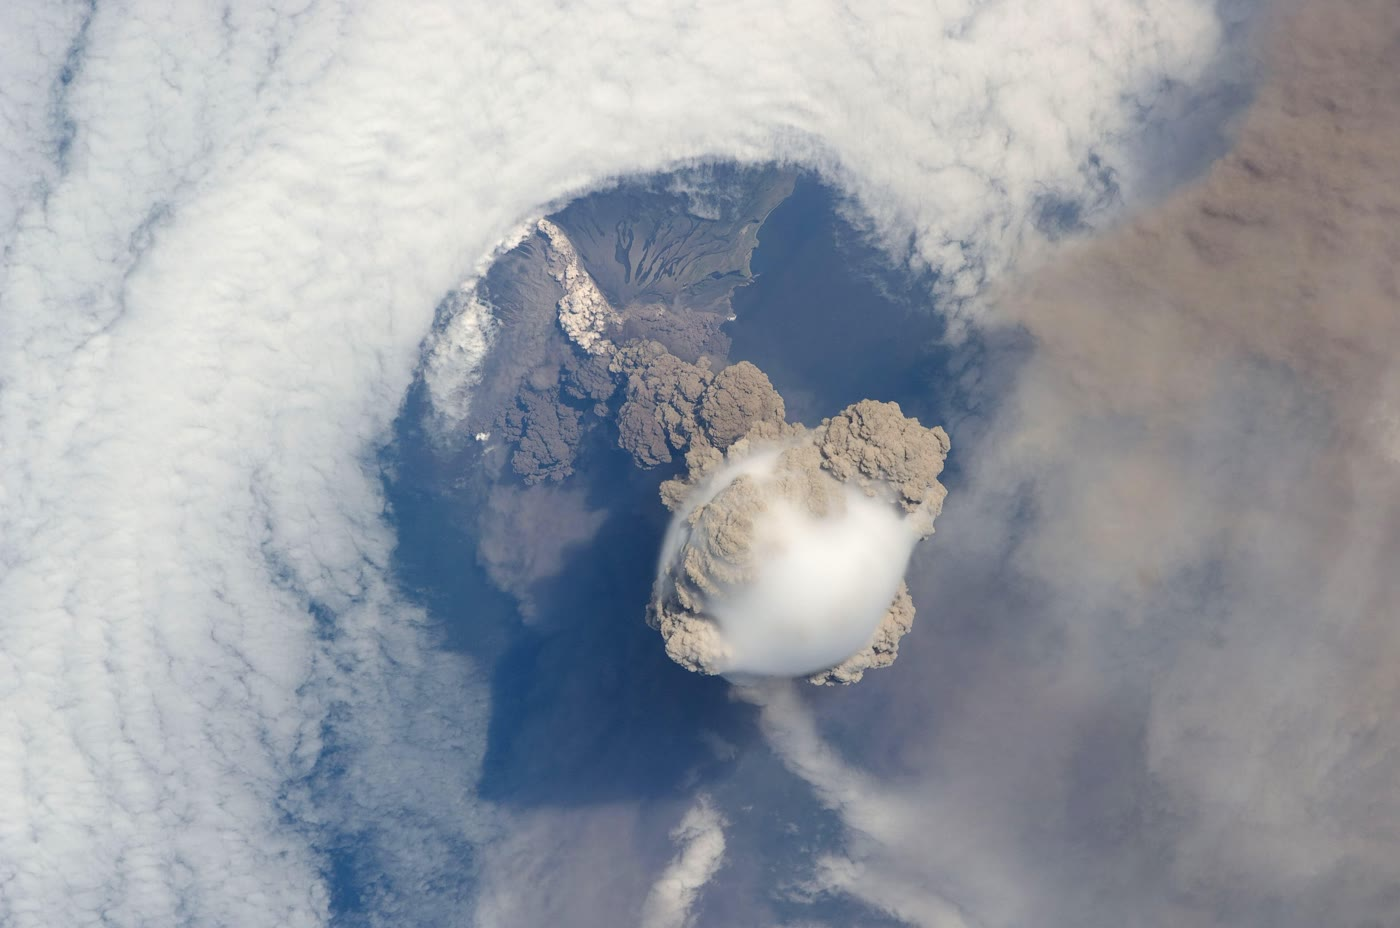
\includegraphics[width=0.66\linewidth]{images/book3/b1-sarychev-iss.jpg}
\par\smallskip{\small Le pic Sarytchev, un volcan de l'arc des Kouriles sur l'île
Matoua, à un stade précoce d'éruption le 12 juin 2009, vu de la
Station spatiale internationale à travers un trou dans les nuages. Des cendres grises, probablement
une coulée pyroclastique, descendent du sommet, et une coiffe lisse de nuage, un
pileus, coiffe la colonne qui monte~; les cendres de l'éruption ont été détectées à plus
de \qty{2400}{km}. Photographie~: NASA, domaine public (Wikimedia
Commons).}
\label{fig:b1:active-margins:sarychev}
\end{omfigure}
% ledger: nasa:sarychev, commons:sarychev

La \omterm{def:b1:layered-earth:layers}{croûte} sous les arcs est épaissie à la fois par raccourcissement et par le magma ajouté
par en dessous~; sous les arcs construits sur des continents, comme les Andes, elle est
parmi les plus épaisses de la Terre.

Derrière certains arcs la plaque chevauchante est étirée. Dan Karig a expliqué
ces bassins marginaux du Pacifique occidental dans le cadre de la tectonique des plaques, en 1971~:
quand le panneau plonge fortement et recule, la fosse et l'arc migrent
vers la plaque qui plonge, et la plaque derrière eux est étirée jusqu'à ce qu'elle
se fende, laissant parfois un arc résiduel éteint du côté opposé. Dans le modèle de plaques
utilisé plus haut, l'expansion d'arrière-arc se fait à environ \qty{32}{mm.an^{-1}} dans le
bassin des Mariannes vers \ang{18}\,N, et à plus de \qty{110}{mm.an^{-1}} dans le
nord du bassin de Lau, derrière Tonga. Là où le panneau est peu incliné, au
contraire, il entraîne la plaque chevauchante, dont la \omterm{def:b1:layered-earth:layers}{croûte} est raccourcie et
épaissie derrière l'arc, comme derrière les Andes.
% ledger: karig:marginal-basins, data:pb2002 (ridge_budget.py: Mariana 32.4, Lau 117.5 mm/yr)

\begin{inthefield}[Alerter d'un tsunami]
Un centre d'alerte aux tsunamis dispose de minutes. En 2011 la première alerte pour la côte
du nord-est du Japon est venue environ trois minutes après le séisme, à partir d'une
magnitude fondée sur les ondes sismiques de courte période~; pour les séismes de
magnitude 8 ou plus une telle magnitude est sous-estimée, et la hauteur du
tsunami l'a été aussi. La magnitude de moment, qui ne sature pas, a pris environ
quinze minutes~: les sismomètres à large bande du Japon avaient été poussés au-delà de
leur étendue de mesure. Depuis 2013, quand la taille d'un séisme aussi grand est incertaine,
la première alerte suppose le plus grand séisme possible en ce lieu et décrit
le tsunami par des mots, comme «~énorme~», plutôt que par un nombre, et les
prévisions s'appuient sur des mesures au large de la mer elle-même, par des bouées
positionnées par satellite et des capteurs de pression au fond de la mer, qui voient la
vague avant qu'elle atteigne la côte.
% ledger: jma:warning

\smallskip
\begin{center}
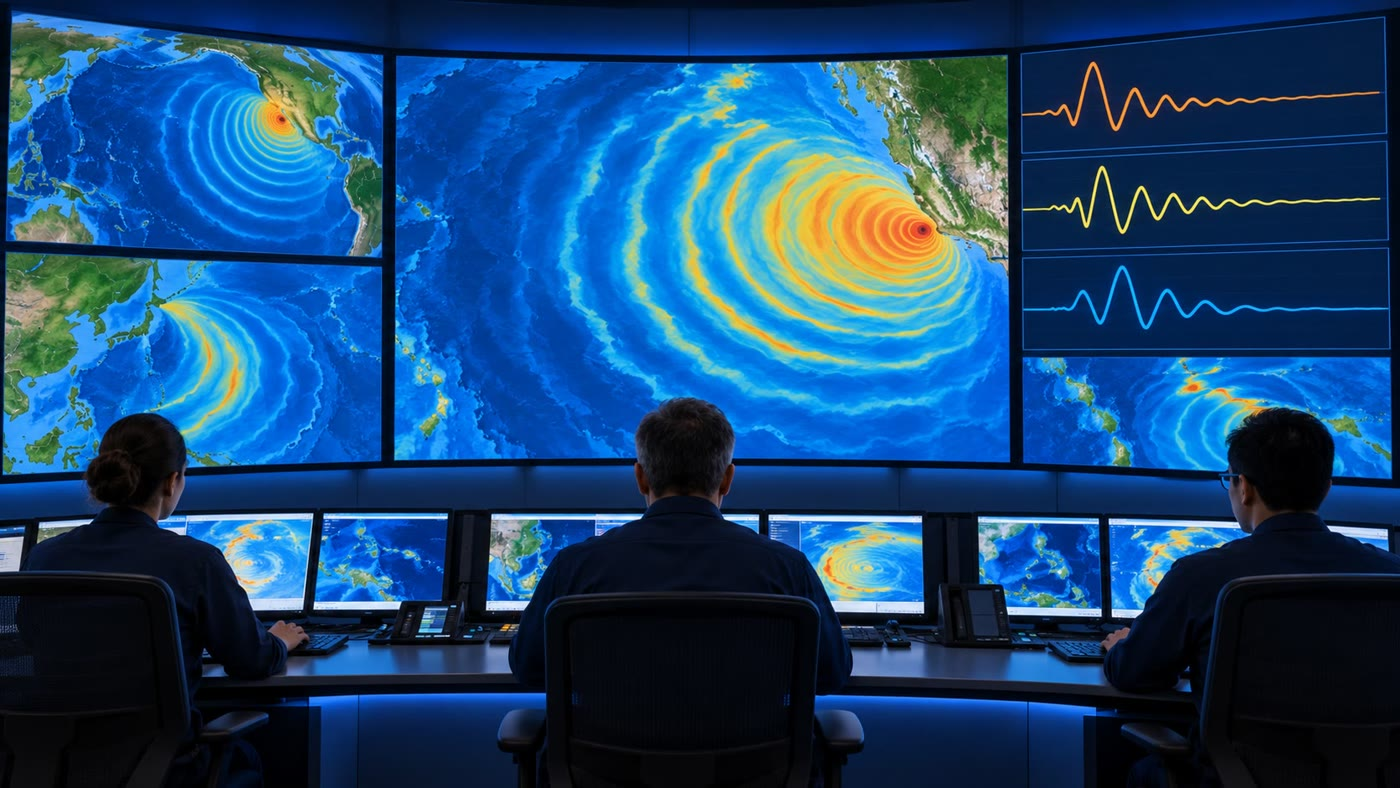
\includegraphics[width=0.7\linewidth]{images/book3/ai/b1-tsunami-centre.jpg}

{\scriptsize Des officiers de permanence dans un centre d'alerte aux tsunamis, devant des écrans
de fronts d'onde calculés et d'enregistrements du niveau de la mer (illustration générée par IA).}
\end{center}
\end{inthefield}

\section{Exercices}

\begin{exercise}[$\star$]\label{exo:b1:active-margins:1}
Une fosse se trouve à \qty{3}{km} sous le plancher océanique qui l'entoure. (a) Si elle n'était pas
compensée, de combien la roche manquante, de masse volumique
\qty{2700}{kg.m^{-3}}, remplacée par de l'eau de mer de masse volumique \qty{1000}{kg.m^{-3}},
abaisserait-elle la pesanteur en ce lieu~? Utiliser la plaque de Bouguer, avec
$G = \qty{6.674e-11}{m^3.kg^{-1}.s^{-2}}$. (b) Comparer à l'anomalie observée
au-dessus de la fosse des Kouriles, environ \qty{-260}{\milli\gal}, où la fosse
se trouve à \qty{3.5}{km} sous le plancher qui l'entoure~: refaire le calcul pour cette
profondeur. (c) Pourquoi l'eau d'une fosse large de dizaines de kilomètres seulement donne-t-elle
moins que la formule de la plaque, et où doit se trouver le reste du déficit~?
\end{exercise}

\begin{exercise}[$\star$]\label{exo:b1:active-margins:2}
La plaque pacifique entre dans la fosse des Kouriles à \qty{82}{mm.an^{-1}}. (a) Quelle
longueur de plaque descend en 10 millions d'années~? (b) Si le panneau s'enfonçait selon un
chemin rectiligne de \omterm{def:b1:geological-maps:attitude}{pendage} \ang{45}, à quelle profondeur serait alors son bord avant~? (c)
Combien de temps met-il à atteindre \qty{600}{km}~?
\end{exercise}

\begin{exercise}[$\star$]\label{exo:b1:active-margins:3}
Des volcans se dressent au-dessus de l'endroit où un panneau rectiligne est à \qty{110}{km} de profondeur.
Calculer la \omterm{def:b1:active-margins:volcanic-arc}{distance arc--fosse} pour un panneau de \omterm{def:b1:geological-maps:attitude}{pendage} \ang{30}, \ang{45} et
\ang{60}. Quel arc est le plus éloigné de sa fosse~?
\end{exercise}

\begin{exercise}[$\star$]\label{exo:b1:active-margins:4}
Dans le modèle numérique de plaques du chapitre, environ \qty{2.7}{km^2} de plancher
océanique descendent chaque année aux limites de subduction, sur environ
\qty{51000}{km}, et environ \qty{3.0}{km^2} sont faits sur environ
\qty{67000}{km} de dorsales d'expansion. (a) Calculer la vitesse moyenne de convergence et
la vitesse totale moyenne d'expansion, en \unit{mm.an^{-1}}. (b) Sur toutes ses
limites le modèle détruit autant d'aire qu'il en fait. Où va le reste du
nouveau plancher~?
% ledger: data:pb2002 (ridge_budget.py: 2.739 km2 over 51471 km; 3.009 km2 over 67340 km; all 3.511 vs 3.519)
\end{exercise}

\begin{exercise}[$\star\star$]\label{exo:b1:active-margins:5}
Quatre séismes d'une coupe sont en $(x, z) = (200, 150)$, $(300, 250)$,
$(400, 330)$ et $(500, 430)$, en kilomètres. (a) Ajuster la droite du panneau par les moindres
carrés et donner son \omterm{def:b1:geological-maps:attitude}{pendage}. (b) Où la droite atteint-elle la surface~? (c)
Comparer avec le \omterm{def:b1:geological-maps:attitude}{pendage} de la droite passant par les premier et dernier séismes seulement.
\end{exercise}

\begin{exercise}[$\star\star$]\label{exo:b1:active-margins:6}
Un panneau modèle plonge de \ang{25} depuis la fosse jusqu'à \qty{50}{km}, puis de
\ang{45}. Le front volcanique se tient là où le panneau est à \qty{110}{km} de profondeur. (a)
Calculer la \omterm{def:b1:active-margins:volcanic-arc}{distance arc--fosse}. (b) Comparer avec un panneau de \omterm{def:b1:geological-maps:attitude}{pendage} \ang{45} sur toute
la longueur. (c) Le segment profond, prolongé vers le haut, atteint la surface~: où~? Comparer
avec la droite des Kouriles, qui l'atteint à \qty{53}{km} de la fosse vers l'intérieur des terres. (d)
Quelle distance donnerait un segment profond de \ang{60}~?
\end{exercise}

\begin{exercise}[$\star\star$]\label{exo:b1:active-margins:7}
(a) D'après la proposition de la coque pliée, quel rayon angulaire, et quel rayon en
kilomètres ($R = \qty{6371}{km}$), un arc doit-il avoir au-dessus d'un panneau de \omterm{def:b1:geological-maps:attitude}{pendage}
\ang{45}~? \ang{30}~? \ang{70}~? (b) Quels arcs sont les plus fortement courbés~? (c)
Le panneau des Kouriles plonge de \ang{44.9} et la fosse des Kouriles s'ajuste à un cercle de
\ang{21.9}~: calculer l'écart relatif à la prédiction.
\end{exercise}

\begin{exercise}[$\star\star$]\label{exo:b1:active-margins:8}
Prendre une conductivité de \qty{2.5}{W.m^{-1}.K^{-1}} et une température de surface
de \qty{10}{\celsius}. (a) Calculer le gradient de température en surface sous un
\omterm{def:b1:active-margins:active-margin}{avant-arc} qui perd \qty{35}{mW.m^{-2}} et sous un arrière-arc qui perd
\qty{80}{mW.m^{-2}}. (b) En extrapolant linéairement ces gradients, estimer la
température à \qty{30}{km} dans chacun. (c) Les \omterm{def:b1:layered-earth:discontinuity}{Mohos} d'arrière-arc sont mesurés à 800 à
\qty{900}{\celsius}. Pourquoi l'estimation linéaire est-elle trop élevée~?
% ledger: hyndman:backarc (back-arc 70-85, Moho 800-900); the forearc value is an exercise value
\end{exercise}

\begin{exercise}[$\star\star$]\label{exo:b1:active-margins:9}
Dans le modèle de plaques du chapitre, le bassin des Mariannes s'ouvre près de \ang{18}\,N à
une vitesse totale d'environ \qty{32}{mm.an^{-1}}. (a) Exprimer cette vitesse en
\unit{km.\Ma^{-1}}, et donner la demi-vitesse si l'expansion est symétrique.
(b) Combien de temps le bassin mettrait-il à s'ouvrir de \qty{100}{km} à cette vitesse~?
(c) Donner deux raisons pour lesquelles l'âge d'un \omterm{def:b1:active-margins:active-margin}{bassin d'arrière-arc} ne peut simplement se lire
à partir de sa largeur et de sa vitesse actuelle.
% ledger: data:pb2002 (ridge_budget.py: mariana_18n_mm_yr 32.4)
\end{exercise}

\begin{exercise}[$\star\star\star$]\label{exo:b1:active-margins:10}
Un panneau épais de \qty{100}{km} plonge à \qty{82}{mm.an^{-1}} selon un chemin de \omterm{def:b1:geological-maps:attitude}{pendage}
\ang{45}. Prendre $\kappa = \qty{e-6}{m^2.s^{-1}}$. (a) Combien de temps met-il à
atteindre \qty{600}{km}~? (b) Sur quelle distance la chaleur diffuse-t-elle en lui pendant ce temps, par
$\sqrt{\kappa t}$~? (c) Combien de temps la chaleur mettrait-elle à atteindre son milieu~? (d)
Conclure sur la température du panneau à \qty{600}{km} et sur ses
séismes.
\end{exercise}

\begin{exercise}[$\star\star\star$]\label{exo:b1:active-margins:11}
Un \omterm{def:b1:active-margins:accretionary}{prisme d'accrétion} modèle a une coupe triangulaire~: sa surface s'incline de
$\alpha = \ang{4}$ vers la fosse et sa base plonge de $\beta = \ang{6}$
sous lui, les deux se rejoignant à son front~; il garde ces angles en croissant. (a)
Montrer que son aire est $A = \frac12 L^2(\tan\alpha + \tan\beta)$ pour une largeur
$L$, quand les angles sont assez petits pour que la hauteur à l'arrière soit
$L(\tan\alpha + \tan\beta)$. (b) Des sédiments épais de \qty{1}{km} arrivent sur une plaque
qui converge à \qty{40}{mm.an^{-1}}, et tous sont accrétés~: calculer la
largeur après 1, 4 et 10 millions d'années. Comment $L$ croît-il avec le temps~? (c) Et
si la moitié des sédiments descend avec le panneau~?
\end{exercise}

\begin{exercise}[$\star\star\star$]\label{exo:b1:active-margins:12}
(a) Montrer que la droite des moindres carrés passe par le point moyen
$(\bar x, \bar z)$. (b) Un catalogue donne chaque profondeur \qty{10}{km} trop profonde.
Comment la pente et l'ordonnée à l'origine de la droite ajustée changent-elles~? (c) Les distances
$x$ sont toutes mesurées depuis un point de fosse placé \qty{20}{km} trop loin vers
l'intérieur des terres, de sorte que chaque $x$ est trop petit de \qty{20}{km}. Comment la pente et
l'ordonnée à l'origine changent-elles~? (d) L'une ou l'autre erreur change-t-elle le \omterm{def:b1:geological-maps:attitude}{pendage}~?
\end{exercise}

\section{Problème~: Lire une zone de subduction à partir de ses séismes}

\begin{problem}[{Problème du week-end --- le panneau des Kouriles à partir de huit séismes, à quelle
vitesse il descend, ce que disent sa pesanteur et son flux de chaleur, et où ses volcans
devraient se dresser}]
\label{pb:b1:active-margins:1}
% values: calc/ch14.py; the eight events are real (USGS catalogue, rounded to the km)
% from figdata/out/bachelor-1-slab_seismicity-section.dat
% ledger: data:b3-usgs-kuril, data:pb2002, data:b2-seafloor-age, syracuse:arc-depth, frank:arcs,
% data:b3-grav-kuril, parsons:plate-model, hyndman:backarc; the forearc heat flow is an exercise value
Huit séismes du panneau des Kouriles, tous plus profonds que \qty{70}{km}, sont listés
par leur distance $x$ à la fosse le long de la ligne de coupe, vers la mer
d'Okhotsk, et leur profondeur $z$, toutes deux arrondies au kilomètre.

\begin{center}
\small
\begin{tabular}{lcccccccc}
\hline
séisme & 1 & 2 & 3 & 4 & 5 & 6 & 7 & 8\\
$x$ (\unit{km}) & 155 & 222 & 305 & 319 & 431 & 533 & 578 & 609\\
$z$ (\unit{km}) & 96 & 169 & 245 & 272 & 389 & 489 & 518 & 573\\
magnitude & 5.5 & 5.1 & 5.0 & 5.4 & 5.3 & 5.3 & 5.2 & 6.4\\
\hline
\end{tabular}
\end{center}

\medskip
\noindent\textbf{Partie I --- La droite du panneau.}
\begin{enumerate}
  \item Tracer les huit séismes à la même échelle sur les deux axes, la profondeur
        vers le bas.
  \item Calculer $\sum x_i$, $\sum z_i$, $\sum x_i^2$, $\sum x_i z_i$ et les
        moyennes $\bar x$ et $\bar z$.
  \item Calculer $S_{xx}$ et $S_{xz}$, puis la pente de la droite des moindres carrés
        à trois décimales et son ordonnée à l'origine à une décimale.
  \item Quel est le \omterm{def:b1:geological-maps:attitude}{pendage} du panneau~?
  \item Où la droite atteint-elle la surface~? Qu'est-ce que cela dit de la
        forme du panneau près de la fosse~?
  \item Calculer l'écart $z_i - (a + s x_i)$ de chaque séisme. Lesquels se trouvent le
        plus loin de la droite, et de combien~?
\end{enumerate}

\medskip
\noindent\textbf{Partie II --- À quelle vitesse le panneau descend.} Au début de la
coupe le modèle PB2002 donne une convergence de \qty{87.4}{mm.an^{-1}}~: par rapport
à la plaque d'Okhotsk, la plaque pacifique se déplace vers l'\omterm{def:b1:spherical-astronomy:horizontal}{azimut} \ang{300}. La
ligne de coupe, perpendiculaire à la fosse, court vers l'\omterm{def:b1:spherical-astronomy:horizontal}{azimut} \ang{320.9}.
\begin{enumerate}[resume]
  \item Calculer l'angle entre la convergence et la ligne de coupe, puis
        les composantes de la convergence perpendiculaire et parallèle à la
        fosse.
  \item Quelle longueur de plaque descend dans la fosse en 10 millions d'années~?
  \item Avec le \omterm{def:b1:geological-maps:attitude}{pendage} de la question 4 (arrondi à \ang{45}), combien de temps
        le panneau met-il à porter un point de son sommet de la fosse jusqu'au
        séisme le plus profond de la bande, \qty{632}{km}~? Négliger le \omterm{def:b1:geological-maps:attitude}{pendage} plus
        doux près de la fosse.
  \item La plaque a environ \qty{122}{\Ma} à la fosse. Quel âge a le
        plancher marin qui est maintenant à \qty{632}{km} de profondeur~?
  \item Par $\sqrt{\kappa t}$, avec $\kappa = \qty{e-6}{m^2.s^{-1}}$, sur quelle distance
        la chaleur a-t-elle diffusé dans le panneau pendant cette descente~? Comparer à son
        épaisseur, environ \qty{100}{km}.
\end{enumerate}

\medskip
\noindent\textbf{Partie III --- Pesanteur et flux de chaleur.} Prendre une conductivité de
\qty{2.5}{W.m^{-1}.K^{-1}}.
\begin{enumerate}[resume]
  \item Le vieux plancher océanique devant la fosse perd environ
        \qty{43}{mW.m^{-2}}, l'arrière-arc environ \qty{80}{mW.m^{-2}}~; prendre
        \qty{35}{mW.m^{-2}} pour l'\omterm{def:b1:active-margins:active-margin}{avant-arc}. Calculer le gradient de température
        près de la surface de chacun.
  \item Expliquer pourquoi l'\omterm{def:b1:active-margins:active-margin}{avant-arc} perd moins de chaleur que le vieux plancher océanique
        devant lui.
  \item L'\omterm{def:b1:isostasy-gravity:anomalies}{anomalie à l'air libre} au-dessus de la fosse des Kouriles est d'environ
        \qty{-260}{\milli\gal}. Quelle épaisseur de roche, plus dense que l'eau de \qty{1700}{kg.m^{-3}},
        une plaque de Bouguer demanderait-elle pour donner ce déficit~?
        Comparer avec la profondeur de la fosse sous le plancher qui l'entoure,
        environ \qty{3.5}{km}.
  \item Supposons maintenant que toute la plaque soit enfoncée de \qty{3.5}{km}~:
        l'eau prend la place de la roche à son sommet, et sa \omterm{def:b1:layered-earth:layers}{croûte} prend la
        place du \omterm{def:b1:layered-earth:layers}{manteau} à sa base, de sorte qu'en tout du \omterm{def:b1:layered-earth:layers}{manteau} de masse volumique
        \qty{3300}{kg.m^{-3}} est remplacé par de l'eau. Calculer l'anomalie de la
        plaque de Bouguer. Pourquoi la vraie fosse, large de dizaines de kilomètres seulement, donne-t-elle
        moins~?
  \item La fosse et le bombement externe ne sont pas en équilibre isostatique. Qu'est-ce qui
        les en maintient écartés~?
\end{enumerate}

\medskip
\noindent\textbf{Partie IV --- Où les volcans devraient se dresser.} Utiliser la droite
de la question 3, avec sa pente et son ordonnée à l'origine arrondies.
\begin{enumerate}[resume]
  \item Le premier volcan de la bande est à \qty{164}{km} de la fosse. À quelle profondeur
        est le panneau sous lui~?
  \item Cette profondeur est-elle dans l'intervalle trouvé sous les arcs, 72 à
        \qty{173}{km}~? À quelle distance est-elle de la moyenne, \qty{105}{km}~?
  \item À quelle distance de la fosse le panneau est-il à \qty{100}{km} de profondeur~?
  \item D'après la proposition de la coque pliée, quel rayon angulaire l'arc des
        Kouriles devrait-il avoir, et quel rayon en kilomètres~?
  \item La fosse des Kouriles s'ajuste à un \omterm{def:b1:spherical-astronomy:spherical-triangle}{petit cercle} de \ang{21.9}. Comparer.
  \item Les volcans d'arc se dressent, en moyenne, là où le panneau est à environ
        \qty{105}{km} de profondeur. À quelle distance de la fosse la droite du panneau
        atteint-elle cette profondeur~?
  \item Comparer cette distance à la valeur observée de \qty{164}{km}~: de combien de
        kilomètres et de quelle fraction diffère-t-elle~?
  \item Au kilomètre près, quelle \omterm{def:b1:active-margins:volcanic-arc}{distance arc--fosse} la droite du panneau des Kouriles
        prédit-elle pour des volcans se dressant au-dessus du panneau à \qty{105}{km}~?
\end{enumerate}
\end{problem}
